\cleardoublepage

\chapter{Introducción}
\label{makereference}

Este proyecto tiene como objetivo predecir, a través de herramientas informáticas, la radiación solar en un punto teniendo en cuenta factores geográficos y meteorológicos.

% Mirar descripción inicial TFG y Drive

\begin{figure}[htb]%t=top, b=bottom, h=here
	
	\begin{center}
		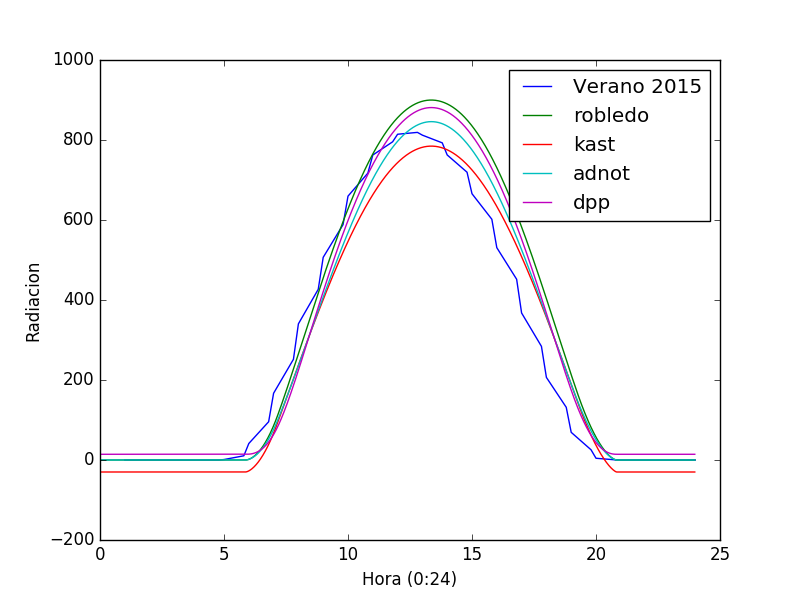
\includegraphics[height=2.5in]{figures/verano2015.png}
		\caption{Modelo verano 2015}
	\end{center}
    
    \label{figure1}
\end{figure}

% +--------------------------------------------------------------------+
% |To create cross-references to figures, tables and segments
% |of text, LaTeX provides the following commands:
% |   \label{marker}
% |   \ref{marker}
% |   \pageref{marker}
% | where {marker} is a unique identifier.
% |
% | In the line above, we use \label{figure1} to mark a location
% | we wish to refer to later.  LATEX replaces \ref by the number of
% | the chapter, section, subsection, figure, or table after which the
% | corresponding \label command was issued. \pageref prints the page
% | number of the page where the \label command occurred.
% |
% +--------------------------------------------------------------------+

\section{Motivación}
\label{makereference1.1}

En un principio decidimos hablar con nuestro futuro tutor de TFG, ya que habíamos tenido una muy buena experiencia como alumnos en su clase de Sistemas Operativos.
Nos propuso tres proyectos distintos: Control de temperatura en máquinas frigoríficas, control de accesos a grandes instituciones y este.

Nos decantamos por este proyecto debido a que nos pareció el más completo en cuanto a tecnologías a manejar y con el que más prodríamos aprender. Mucha implicación tanto hardware, como software. Queríamos hacer algo fuera de lo estudiado en la carrera.

Este proyecto nos ha supuesto aprender lenguajes que no conocíamos (python y matlab), reforzar otros (bash).

Además de todo esto, hace dos años cursamos una asignatura optativa llamada Minería de datos y el paradigma Big Data, la cual nos motivó bastante a la hora de elegir este proyecto. Nos gustaba mucho la idea de aprender algo de 'Machine Learning' y Python debido a que es un sector muy puntero y solicitado.

% Referenciar
In this paragraph, we want to refer to Fig.~\ref{figure1}
mentioned at the beginning of this chapter.  We also refer to the
Table~\ref{table1}.

\section{Breve descripción del sistema}
\label{makereference1.2}

Este sistema cuenta con cuatro grandes módulos de trabajo para llevar a cabo su función: nodo, servidor de datos, servidor de resultados y visualizador de datos.

El \textbf{nodo}, encargado de recoger los datos necesarios, está formado por distintos sensores que recogen la información meteorológica necesaria y una pequeña placa programable encargada de enviar esta información al \textbf{servidor de datos}.

El \textbf{servidor de datos}, es el encargado de recibir, almacenar y distribuir la información obtenida por el \textbf{nodo}. 

El \texbf{servidor de resultados} tiene como función recoger la información almacenada del servidor de datos, procesarla para obtener la predicción y enviarla al \textbf{visualizador de datos}.

El visualizador de datos es otro sistema encargado de obtener toda la información resultante del proceso anterior y presentarla al usuario de forma clara y precisa.

In this section, we refer back to text mentioned in
Section~\ref{makereference1.1} on page~\pageref{makereference1.1}.

\section{Making a Citation}
\label{makereference1.3}

Here's an example of a citation to a single
work.~\cite{CT:Weiner:1999} It's also possible to make multiple
citations.~\cite{CT:Phillips:1985, ARP:Loy:1974}
